%%%%%%%%%%%%%%%%%%%%%%%%%%%%%%%%%%%%%%%%%
% Journal Article
% LaTeX Template
% Version 1.3 (9/9/13)
%
% This template has been downloaded from:
% http://www.LaTeXTemplates.com
%
% Original author:
% Frits Wenneker (http://www.howtotex.com)
%
% License:
% CC BY-NC-SA 3.0 (http://creativecommons.org/licenses/by-nc-sa/3.0/)
%
%%%%%%%%%%%%%%%%%%%%%%%%%%%%%%%%%%%%%%%%%

%----------------------------------------------------------------------------------------
%	PACKAGES AND OTHER DOCUMENT CONFIGURATIONS
%----------------------------------------------------------------------------------------

\documentclass[twoside]{article}

\usepackage{lipsum} % Package to generate dummy text throughout this template
\usepackage[french]{babel}

\usepackage[utf8]{inputenc}

\usepackage[sc]{mathpazo} % Use the Palatino font
\usepackage[T1]{fontenc} % Use 8-bit encoding that has 256 glyphs
\linespread{1.05} % Line spacing - Palatino needs more space between lines
\usepackage{microtype} % Slightly tweak font spacing for aesthetics

\usepackage[hmarginratio=1:1,top=32mm,columnsep=20pt]{geometry} % Document margins
\usepackage{multicol} % Used for the two-column layout of the document
\usepackage[hang, small,labelfont=bf,up,textfont=it,up]{caption} % Custom captions under/above floats in tables or figures
\usepackage{booktabs} % Horizontal rules in tables
\usepackage{float} % Required for tables and figures in the multi-column environment - they need to be placed in specific locations with the [H] (e.g. \begin{table}[H])
\usepackage{hyperref} % For hyperlinks in the PDF

\usepackage{lettrine} % The lettrine is the first enlarged letter at the beginning of the text
\usepackage{paralist} % Used for the compactitem environment which makes bullet points with less space between them

\usepackage{abstract} % Allows abstract customization
\renewcommand{\abstractnamefont}{\normalfont\bfseries}
\renewcommand{\abstractname}{Résumé} % Set the "Abstract" text to bold
\renewcommand{\abstracttextfont}{\normalfont\small\itshape} % Set the abstract itself to small italic text

\usepackage{titlesec} % Allows customization of titles
\renewcommand\thesection{\Roman{section}} % Roman numerals for the sections
\renewcommand\thesubsection{\arabic{subsection}.\arabic{subsection}} % Roman numerals for subsections
\titleformat{\section}[block]{\bfseries\large\scshape\centering}{\thesection.}{1em}{} % Change the look of the section titles
\titleformat{\subsection}[block]{\bfseries\large}{\thesubsection.}{1em}{} % Change the look of the section titles

\usepackage{fancyhdr} % Headers and footers
\pagestyle{fancy} % All pages have headers and footers
\fancyhead{} % Blank out the default header
\fancyfoot{} % Blank out the default footer
\renewcommand{\headrulewidth}{0pt} %pour enlever la ligne du header
%\fancyhead[C]{titre, date, noms...	} % Custom header text
\fancyfoot[RO,LE]{\thepage} % Custom footer text


%agrandissement de la zone de texte
\addtolength{\oddsidemargin}{-1cm}
\addtolength{\evensidemargin}{-1cm}
\addtolength{\textwidth}{2cm}

%pour les maths
\usepackage{amsmath}
\usepackage{amsfonts}

%pour les figures
\usepackage{graphicx}
\usepackage{caption}
\usepackage{subcaption}

\renewcommand{\degre}{$^{\circ}$}

%----------------------------------------------------------------------------------------
%	TITLE SECTION
%----------------------------------------------------------------------------------------

\title{\vspace{-15mm}\fontsize{24pt}{10pt}\selectfont\textbf{Étude de la propagation des ondes de volume et de surface dans une plaque}} % Article title

\author{
\large
{Alice \textsc{Dinsenmeyer} \& Thomas \textsc{Lechat}}\\[2mm] % Your name %\thanks{}
%\normalsize University of California \\ % Your institution
%\normalsize \href{mailto:john@smith.com}{john@smith.com} % Your email address
\vspace{-5mm}
}
\date{}

%----------------------------------------------------------------------------------------

\begin{document}

\maketitle % Insert title

\thispagestyle{fancy} % All pages have headers and footers

%----------------------------------------------------------------------------------------
%	ABSTRACT
%----------------------------------------------------------------------------------------

\begin{abstract}

\noindent Ce rapport revient sur trois types d'ondes se propageant dans les solides : transversale, longitudinale et de Rayleigh. La vitesse de ces ondes est mesurée dans une plaque d'alliage d'aluminium, à l'aide de transducteurs mono-éléments piézoélectriques. Les ondes de Rayleigh et longitudinales (L) sont aussi caractérisées par leur atténuation. Il apparaît que les ondes de Rayleigh sont plus atténuées que les ondes L.

\end{abstract}

%----------------------------------------------------------------------------------------
%	ARTICLE CONTENTS
%----------------------------------------------------------------------------------------

\begin{multicols}{2} % Two-column layout throughout the main article text

\section{Introduction}
La caractérisation de matériaux par l'utilisation de transducteurs mono-éléments peut être effectuées par génération de différents types d'onde : des ondes de volumes sont mesurées en "through mode", transmission latérale ou "echo mode" et une onde de surface, l'onde de Rayleigh, est observée en transmission latérale.\\

 Les ondes de Rayleigh sont des ondes se propageant à l'interface entre un matériau semi-infini et le vide. Elles ont été mise en évidence par Lord Rayleigh en 1885 \cite{R} et résultent d'une recombinaison d'ondes longitudinales (L) et transversales (T). Ces ondes sont évanescentes dans le matériau mais permettent quand même le contrôle de défauts subsurfaciques. De plus, elles sont très utilisées en sismologie car elles peuvent être générées lors des tremblements de terres.\\

Ce rapport donne un bref aperçu des caractéristiques de ces ondes, notamment leur vitesse et leur atténuation ainsi que des ondes de volume.


%------------------------------------------------
\subsection*{Notations}

L'excitation normale du transducteur donne naissance à une onde longitudinale dans le sabot en Plexiglas se propageant à un angle $\theta^{i}$ de la normale à la plaque, à la vitesse $c_{plexi}$. Par conversion de mode, une onde longitudinale (L) et une onde transversale (T) sont générées dans la plaque. Ces ondes se propagent formant respectivement les angles $\theta_{plaque}^L$ et $\theta_{plaque}^T$ avec la normale à la plaque, aux vitesses $c_{plaque}^T$ et $c_{plaque}^L$.\\

Le temps de parcours de l'onde incidente dans le sabot est noté $\Delta t_{sabot}$, et celui des ondes L et T dans la plaque sont notés $\Delta t_{plaque}^L$ et $\Delta t_{plaque}^T$. Finalement, si d est l'épaisseur de la plaque, la distance parcourue par les ondes L dans le sabot, puis L et T dans la plaque sont : 
\begin{itemize}
	\item[$\bullet$] $c_{plexi} \times \Delta t_{sabot}$ , \\
	\item[$\bullet$] $c_{plaque}^T \times \Delta t_{plaque}^L = d/\cos(\theta_{plaque}^L)$ , \\
	\item[$\bullet$] $c_{plaque}^L \times \Delta t_{plaque}^T = d/\cos(\theta_{plaque}^T)$.
\end{itemize}

L'ensemble de ces notation est résumé dans la figure~\ref{notations}.

\begin{figure}[H]
	\centering
	\includegraphics[scale=0.23]{notations/dessin.png}
	\includegraphics[scale=0.23]{notations/dessin2.png}
	\caption{\label{notations}Représentation des angles d'incidence et de transmission (à gauche) et des distances parcourues par les ondes (à droite).}
\end{figure}

\section{Ondes de volume}

On cherche a évaluer la vitesse des ondes T et L dans une plaque de d'épaisseur d=20,5 mm, a priori en aluminium. Les mesures sont effectuées à l'aide de  transducteurs piézoélectriques de fréquence centrale 2.5 MHz. Les temps de vols sont relevés directement sur l'oscilloscope. 

\subsection{En incidence normale}

En utilisant un seul transducteur en mode écho (sans sabot), une succession d'écho est observé. Le premier correspond à un temps d'arrivée de 6,6~$\mu$s, ce qui correspond à deux fois le temps de vol dans une épaisseur de la plaque. L'épaisseur de la plaque étant de 20,5 mm, on peut en déduire que la vitesse pour les ondes L dans ce matériau est de $20,5.10^{-3}/3,3.10^{-6}\approx6200$ m/s. Considérant que le coefficient de Poisson de l'aluminium est de 0,35 et que son module d'Young est de 70 GPa, la célérité des ondes L devrait être de 4730 m/s. La plaque semble donc être plutôt faite d'un alliage d'aluminium, beaucoup plus dense que l'aluminium.\\

La même mesure est effectuée avec sabot, en incidence normale, pour évaluer l'épaisseur de ce sabot en Plexiglas utilisé par la suite. Le nouveau temps d'arrivée est 62.4 $\mu$s, ce qui correspond à deux fois le temps de vol dans le sabot puis dans la plaque. On a donc $\Delta t_{sabot} =27,9 \mu$s. Connaissant la vitesse des ondes L dans le Plexiglas ($c_{plexi}=2730$ m/s), on peut en déduire que l'épaisseur d'un sabot est de 38 mm. Cette valeur est vérifiée par une mesure au pied à coulisse.

\subsection{En incidence oblique}
	\subsubsection{Vitesse des ondes T}
	On cherche ici à évaluer la vitesse des ondes T dans la plaque. Pour cela, les mesures sont effectuée en "through mode".
	Le transducteur est incliné à l'aide du sabot de 10$^{\circ}$. Cet angle étant faible, le parcours de l'onde T dans la plaque est considéré égal à l'épaisseur de la plaque. Le temps de vol mesuré $2\times(\Delta t_{sabot}+\Delta t_{plaque}^T)$ du second paquet d'onde correspond au parcours d'une onde L dans les sabots et d'une onde T dans la plaque. La vitesse des ondes T est donc retrouvée grâce à la relation : 
	$$c_{T}^{plaque}=\frac{d}{2(\Delta t_{sabot}+\Delta t_{plaque}^T)-2\Delta t_{sabot}}=2733~ \text{m/s.}$$
	
Cette valeur est légèrement sous-estimée puisque l'angle de transmission n'est en réalité pas nul. L'ordre de grandeur est cependant proche de la valeur théorique de $c_{T}$ qui est de 3100 m/s dans l'aluminium.
	
	\subsection{Évaluation de l'anisotropie}
	On souhaite connaître l'évolution de la vitesse de phase des ondes T et L dans la plaque en fonction de l'angle d'incidence $\theta^{i}$, afin de déterminer l'anisotropie du matériau.\\
	
	Nous avons pour cela, accès aux temps de parcours des ondes dans la plaque $\Delta t_{plaque}$. Reste à connaître l'angle de réfraction $\theta_{plaque}$ dans la plaque, donné par les relations : 
\begin{eqnarray}
		\frac{sin\theta^{i}}{c_{plexi}} &=&\frac{sin\theta^{T}_{plaque}}{c_{plaque}^T} \label{SD}\\ \text{et}~~~~~
		c_{plaque}^T&=&\frac{d}{cos\theta_{plaque}^T. ~\Delta t_{plaque}^T} \label{geom}.	
\end{eqnarray}
Ce qui donne un système de deux équations à deux inconnues ($c_{plaque}^T$ et $\theta_{plaque}$).\\

La relation~\ref{geom} donne : $$\cos\theta_{plaque} = \frac{d}{c_{plaque}. \Delta t_{plaque}}.$$
Et comme, d'après~\ref{SD}, $$c_{plaque} = \frac{sin\theta_{plaque}.c_{plexi}}{sin\theta^{i}},$$ on a donc 
\begin{eqnarray*}
\cos\theta^{T}_{plaque}&=& \frac{d.\sin\theta^{i}}{\Delta t_{plaque}.sin\theta_{plaque}.c_{plexi}}\\
	\Leftrightarrow  \frac{\sin2\theta_{plaque}}{2}& = &\frac{d.\sin\theta^{i}}{\Delta t_{plaque}.c_{plexi}}\\
	\Leftrightarrow \theta_{plaque} &=& \frac{1}{2}\arcsin\left(\frac{2d.\sin\theta^{i}}{\Delta t_{plaque}.c_{plexi}}\right)
\end{eqnarray*}

Il semble qu'il ne soit pas possible de raisonner ainsi, puisque la dernière relation impose que $\theta^{T}_{plaque}\leq 45^{\circ}$, car $-1\leq\arcsin(x) \leq1$. Or on sait que l'angle de transmission des ondes T est susceptible de dépasser 45$^{\circ}$. \\ \quad

Même sans réinjecter dans ces équations les retards mesurés, le tableau~\ref{tab} montre que le temps de parcours pour les deux types d'onde diminue tandis que leur trajet augmente. Il semblerait donc que la plaque soit anisotrope. Cependant, il y a une forte incertitude sur l'angle d'incidence due à l'imprécision du sabot, ce qui met en doute cette supposition.

\begin{table}[H]
	\begin{tabular}{c|c|c|c|c|c}
		$\theta^{i}$ ($^{\circ}$)  & 10 & 30 & 40 & 50 & 60\\ \hline
		$\Delta t_{plaque}^L$ ($\mu$s)& 3.8 & 2.7 & & &   \\ \hline
		$\Delta t_{plaque}^T$ ($\mu$s) &7.5& 6.6 & 6 & 4 & 3.7\\ 
	\end{tabular}
	\caption{Temps de parcours des ondes T et L pour différents angles d'incidence.\label{tab}}
\end{table}

Ce tableau montre aussi qu'il n'y a plus génération d'ondes L au delà de 30\degre et d'onde T au delà de 60\degre.


\section{Ondes de surface}

Quand l'angle d'incidence dépasse ces deux angles critiques, il y a génération d'une onde de surface appelée onde de Rayleigh.
\subsection{Mesure de vitesse}
À l'aide de deux transducteurs, l'onde de Rayleigh est observée en transmission latérale. En effectuant une mesure de retard $\Delta t_R$ pour trois distances inter-transducteurs $L$, on obtient les valeurs de célérité $c_R$ suivantes :

\begin{tabular}{c|c| c | c}
$\Delta t_R$ ($\mu$s) &4.8 & 6.05 & 10.9 \\ \hline
$L$ (mm) & 14.5 & 16.3 & 30.8 \\ \hline
$c_R$ (m/s) &3208 & 2694 & 2826
\end{tabular}

La vitesse des ondes de Rayleigh dans la plaque semble donc légèrement inférieur à 3000 m/s.\\

Une valeur approchée théorique de cette vitesse peut être calculée de cette façon : 
$$c_R=c_{plaque}^T \frac{0.718 - \left(\frac{c_{plaque}^T}{c_{plaque}^L}\right)^2}{0.75 - \left(\frac{c_{plaque}^T}{c_{plaque}^L}\right)^2}=2900 \text{m/s},$$
en prenant $c_{plaque}^T=3100$ m/s et  $c_{plaque}^L=6200$ m/s.
Cette valeur est très proche de celle obtenue expérimentalement.

\subsection{Onde de Rayleigh de fuite}

L'onde de Rayleigh étant une onde de surface, elle peut rayonner dans le fluide en contact avec le son milieu de propagation. Ce rayonnement (appelé onde de Rayleigh de fuite) est plus ou moins important selon la densité et la viscosité du fluide. \\

Par conséquent, si un fluide, du couplant par exemple, se trouve sur le chemin de l'onde mesurée, une forte atténuation peut compromettre son observation. En effet, une grande partie de l'énergie est rayonnée dans ce fluide.

Pour observer le phénomène, il suffit de générer une onde de Rayleigh, puis de la mesurer avec un capteur se trouvant séparé du matériau par une fine couche d'eau. 


\section{Atténuation}
La décroissance des ondes se propageant suivant la direction $x$ est de la forme $e^{-\alpha x)}$. On souhaite déterminer $\alpha$, qui correspond au coefficient d'atténuation.

\subsection{Expérimentalement}
La figure~\ref{attenuation} représente des mesures de Mathieu et Fanon : ~\ref{attenuationL} est une mesure de la propagation des ondes L (excitation en incidence normale) et ~\ref{attenuationR} est une mesure des ondes de Rayleigh se propageant sur 11,4 cm. Ces mesures sont effectuées à 2.25 MHz, avec un transducteur dont la bande passante est centrée autour de cette fréquence.


\begin{figure}[H]
	\centering
	\begin{subfigure}[b]{0.5\textwidth}
	    \centering
        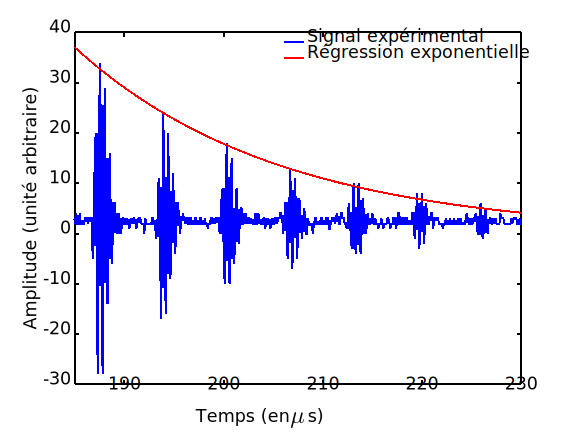
\includegraphics[scale=0.45]{figures/attenuationL.png}
        \subcaption{ondes L en modes écho}
        \label{attenuationL}
    \end{subfigure}\\\vspace{0.5cm}
	\begin{subfigure}[b]{0.5\textwidth}
	    \centering
        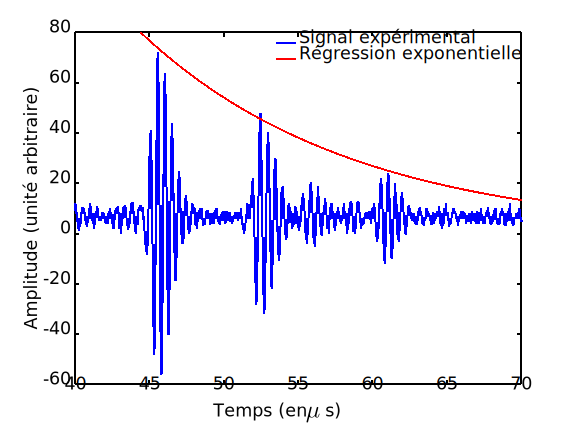
\includegraphics[scale=0.45]{figures/attenuationR.png}       
        \subcaption{ondes de Rayleigh}
        \label{attenuationR}
    \end{subfigure}
	\caption{\label{attenuation}Calcul de l'atténuation par régression, des ondes L (\ref{attenuationL}) et de Rayleigh (\ref{attenuationR}).}
\end{figure}

Après avoir passé les données en dB, une régression linéaire est effectuée. Les coefficients d'atténuation $\alpha_{/s}^{L}$ et $\alpha_{/s}^{R}$ ainsi obtenus représentent la décroissance des ondes L et de Rayleigh par seconde. \\
En divisant ces coefficients par la vitesse des ondes, on obtient donc les atténuations par mètre : 
$$\alpha_{/m}^{L}=\frac{\alpha_{/s}^L}{c_{plaque}^L}=7.8 ~NP/m$$ $$~~~~\text{et}~~~~\alpha_{/m}^{R}=\frac{\alpha_{/s}^R}{c_{R}}=11.3~NP/m.$$

On mesure donc une atténuation plus importante pour les ondes de Rayleigh (10 dB/m) que pour les ondes L (3.4 dB/m).

\section{Conclusion}

Les expérimentations faites dans le cadre de cette étude illustrent les principes généraux liés à la propagation des ondes dans  les solides : 
\begin{itemize}
	\item les vitesses sont telles que : $c_{R}<c_{T}<c_{L}$,
	\item les ondes sont atténuées des quelques dB/m dans les solides à 2.5 MHz, ce qui est faible et avantageux pour le CND,
	\item l'état de surface du solide est un paramètre important en CND car il peut engendrer une forte atténuation des ondes de surface.	
\end{itemize}

\begin{thebibliography}{99} % Bibliography - this is intentionally simple in this template
\bibitem[R]{R}
Lord Rayleigh, 1885 \\
\newblock \emph{ Wave propagated along the plane surface of an elastic solid}
\end{thebibliography}

\end{multicols}

\end{document}
